\documentclass[12pt]{article}
\usepackage[a4paper, margin=2.5cm]{geometry}
\usepackage[utf8]{inputenc}
\usepackage[T1]{fontenc}
\usepackage{setspace}
\onehalfspacing
\usepackage{graphicx}
\usepackage{amsmath, amssymb}
\usepackage{booktabs}
\usepackage{caption}
\usepackage{float}
\usepackage{hyperref}
\usepackage{pgfplots}
\usetikzlibrary{intersections, patterns, decorations.markings, calc}

\title{Econometrics II -- Assignment 2:\\
Geopolitical Risk and Economic Activity}
\date{Spring 2026}

\begin{document}

\maketitle
This paper studies the dynamic relationship between geopolitical risk, stock returns, and U.S. economic activity using a small monthly VAR model. The main question is whether geopolitical risk helps predict stock returns and industrial production growth, whether feedback runs in the opposite direction, and whether there is evidence of contemporaneous comovement.

The analysis uses the benchmark Geopolitical Risk (GPR) index of Caldara and Iacoviello (2022), U.S. industrial production, and U.S. value-weighted stock returns. I estimate a reduced-form VAR, select lag length by information criteria, evaluate misspecification before inference, test Granger-causality restrictions, and interpret orthogonalized impulse responses under a transparent Cholesky ordering with GPR first.

The preferred specification is VAR(1) by BIC. The main empirical finding is that lagged stock returns predict industrial production growth, while lagged GPR does not significantly predict either stock returns or production growth in this three-variable system. A GPR shock lowers stock returns on impact in the orthogonalized IRF, but the effect is short-lived and estimated imprecisely. These conclusions remain qualitatively similar in the post-9/11 sample and when recent crisis years are excluded.

% ─────────────────────────────────────────────────────────────────────────────
\section{Introduction}
% ─────────────────────────────────────────────────────────────────────────────



The dataset contains monthly observations from January 1985 to December 2025 (492 usable observations after transformation). The variables are:
\begin{align*}
g_t &= \log(GPR_t), \\
y_t &= \log(INDPRO_t) - \log(INDPRO_{t-1}), \\
s_t &= \log\!\left(1 + \frac{Mkt_t}{100}\right).
\end{align*}
Hence, $y_t$ is monthly industrial production growth and $s_t$ is continuously compounded monthly stock return.

Figure~\ref{fig:series} shows the three series and major event windows (9/11, COVID-19, 2022 war shock, and recent Middle East escalation). The most pronounced outlier is in industrial production growth during early 2020, and all three series display non-Gaussian crisis behavior. Summary statistics from the notebook confirm this, especially for $y_t$ with very high kurtosis.

\begin{figure}[H]
	\centering
	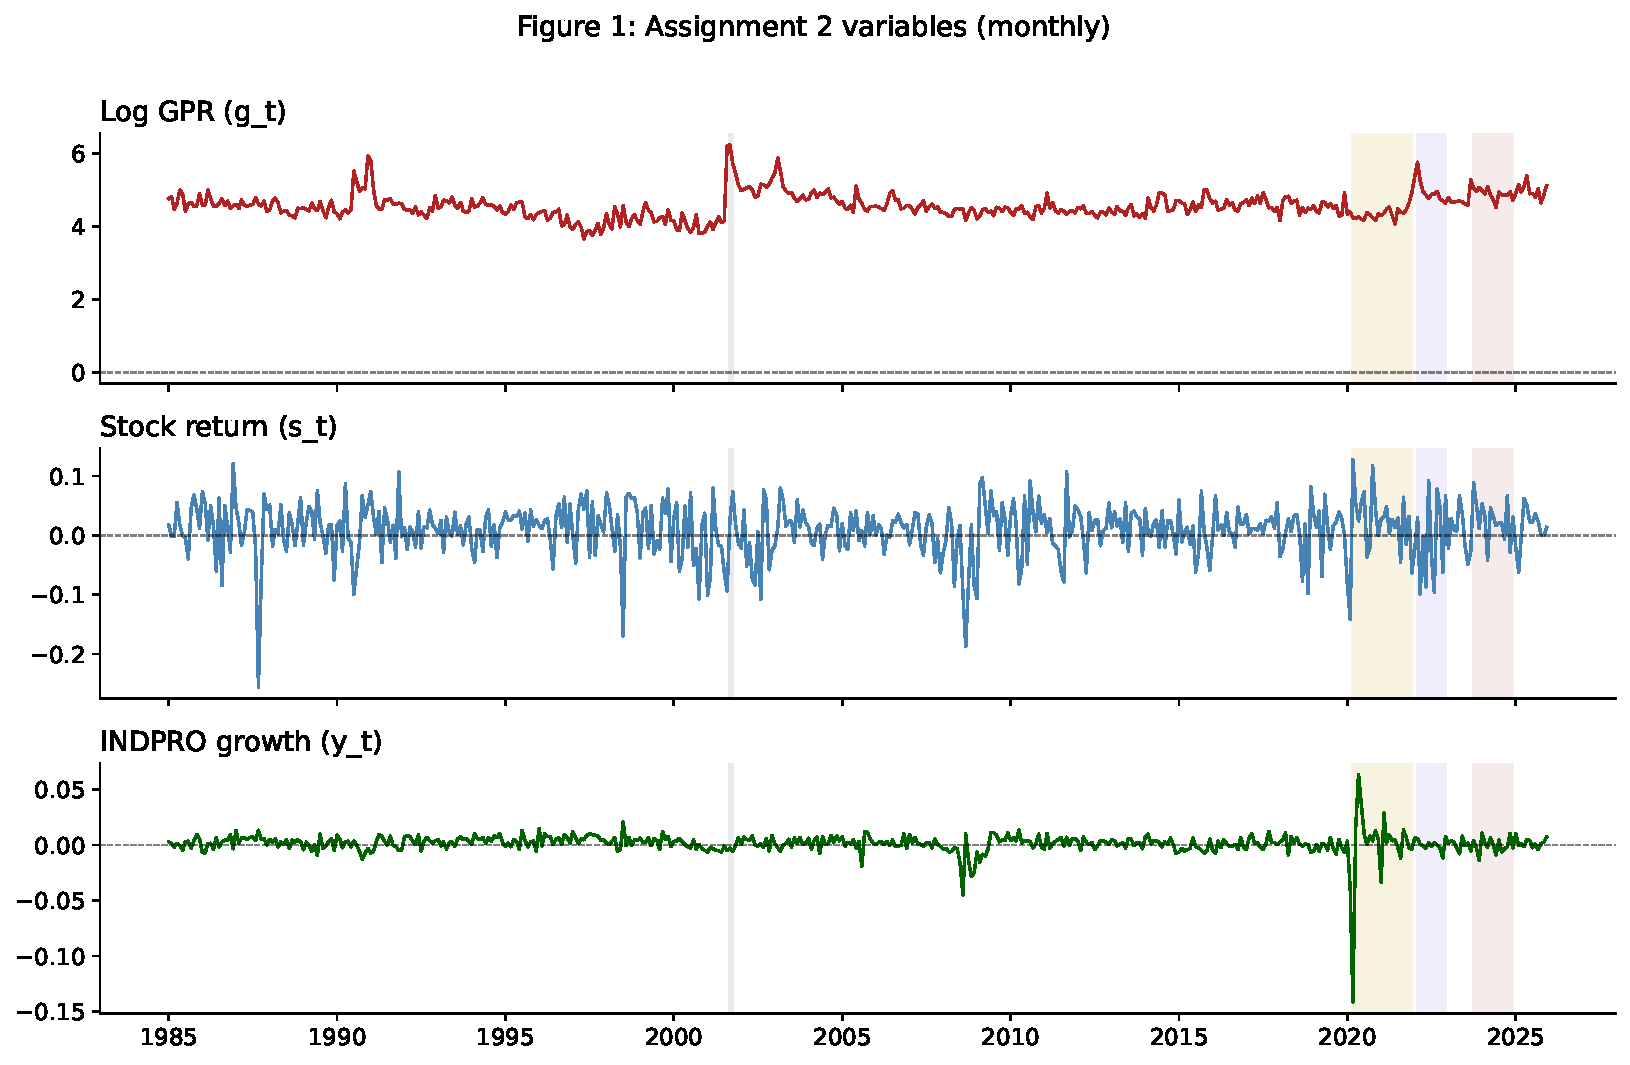
\includegraphics[width=0.95\textwidth]{figures/fig1_series_panel.pdf}
	\caption{Monthly series for $g_t$, $s_t$, and $y_t$ with highlighted event windows.}
	\label{fig:series}
\end{figure}
% ─────────────────────────────────────────────────────────────────────────────
\section{Description of the Data}
% ─────────────────────────────────────────────────────────────────────────────



% ─────────────────────────────────────────────────────────────────────────────
Let $Z_t = (g_t, s_t, y_t)'$. The reduced-form VAR($k$) is
\begin{equation}
Z_t = \mu + \Pi_1 Z_{t-1} + \cdots + \Pi_k Z_{t-k} + e_t,
\end{equation}
with $E[e_t\mid\mathcal{I}_{t-1}] = 0$ and $E[e_t e_t'] = \Omega$.

Under stationarity and standard regularity conditions, equation-by-equation OLS is numerically identical to Gaussian MLE in a VAR. The asymptotic distribution of the coefficient estimator is Gaussian, so Wald/LR tests can be used for linear restrictions. Stability requires all roots of the companion representation to lie outside the unit circle (equivalently, all companion eigenvalues in modulus below one).

For predictive causality, I test block exclusion restrictions in each equation. For example, no Granger causality from $g$ to $s$ in VAR($k$) is
\begin{equation}
H_0: \text{all } k \text{ lag coefficients on } g_{t-j} \text{ in the } s_t \text{ equation are zero}.
\end{equation}
Wald statistics are asymptotically $\chi^2$ under correct specification.

To discuss contemporaneous effects, I use orthogonalized impulse responses based on Cholesky factorization of $\Omega$ with ordering $(g,s,y)$. This imposes one identifying restriction motivated by the assignment context: geopolitical risk does not react contemporaneously within month to stock returns and activity.
\section{Econometric Theory}
% ─────────────────────────────────────────────────────────────────────────────



% ─────────────────────────────────────────────────────────────────────────────
\section{Empirical Analysis}
\subsection{Model Selection and Modeling Progress}

I estimate VAR($k$) for $k=1,2,3,4$ and compare AIC, BIC, and HQIC. Table~\ref{tab:lag_selection} shows that BIC selects VAR(1), while AIC is slightly lower at VAR(3). Following a parsimonious specification rule and the assignment scope, I take VAR(1) as preferred and then evaluate diagnostics before interpretation.

\begin{table}
\caption{VAR lag-order selection.}
\label{tab:lag_selection}
\begin{tabular}{lrrrr}
\toprule
 & AIC & BIC & HQIC & FPE \\
Lag &  &  &  &  \\
\midrule
1 & -18.552500 & -18.449900 & -18.512200 & 0.000000 \\
2 & -18.561500 & -18.381800 & -18.491000 & 0.000000 \\
3 & -18.577200 & -18.320000 & -18.476200 & 0.000000 \\
4 & -18.548300 & -18.213400 & -18.416700 & 0.000000 \\
\bottomrule
\end{tabular}
\end{table}


\subsection{Misspecification Checks}

Table~\ref{tab:diagnostics} reports Ljung-Box, ARCH-LM, and Jarque-Bera tests by equation. Residual autocorrelation is borderline for $g_t$ and clearly present for $y_t$ at lag 12. Heteroskedasticity is not rejected for $g_t$ but is detected for $s_t$ and $y_t$. Normality is strongly rejected in all equations, reflecting crisis outliers.

These results imply caution for textbook Gaussian finite-sample inference. Coefficient estimates remain informative for dynamic patterns, but statistical significance should be interpreted conservatively because residual volatility and tails are nonstandard.

\begin{table}
\caption{Misspecification diagnostics by equation for preferred VAR.}
\label{tab:diagnostics}
\begin{tabular}{lrrrrrr}
\toprule
 & Ljung-Box(12) stat & Ljung-Box(12) p & ARCH-LM(4) stat & ARCH-LM(4) p & Jarque-Bera stat & Jarque-Bera p \\
Equation &  &  &  &  &  &  \\
\midrule
g & 21.162700 & 0.048000 & 0.595200 & 0.963600 & 4505.652900 & 0.000000 \\
s & 10.869900 & 0.540100 & 14.857100 & 0.005000 & 261.660000 & 0.000000 \\
y & 32.157900 & 0.001300 & 28.930200 & 0.000000 & 114320.617100 & 0.000000 \\
\bottomrule
\end{tabular}
\end{table}


The estimated residual correlation matrix indicates modest contemporaneous comovement: $\text{corr}(e_g,e_s)\approx -0.106$, $\text{corr}(e_g,e_y)\approx 0.004$, and $\text{corr}(e_s,e_y)\approx -0.058$.

\subsection{Granger-Causality Results}

Table~\ref{tab:granger} summarizes directional Wald tests. The key findings are:
\begin{itemize}
	\item No evidence that $g_t$ Granger-causes $s_t$ ($p=0.478$) or $y_t$ ($p=0.248$).
	\item No evidence that $s_t$ or $y_t$ Granger-cause $g_t$.
	\item Clear evidence that $s_t$ Granger-causes $y_t$ ($p<0.001$).
\end{itemize}
Hence, in this system, stock returns contain predictive information for future industrial production growth, while lagged geopolitical risk does not add significant predictive content conditional on the included variables.

\begin{table}[H]
\centering
\caption{Granger-causality tests (Wald) in preferred VAR.}
\label{tab:granger}
\begin{tabular}{lrrl}
\toprule
 & Statistic & p-value & Reject 5% \\
\midrule
g -> s & 0.5036 & 0.4779 & No \\
g -> y & 1.3324 & 0.2484 & No \\
s -> g & 0.6413 & 0.4233 & No \\
y -> g & 0.0081 & 0.9282 & No \\
s -> y & 20.5118 & 0.0000 & Yes \\
y -> s & 0.8679 & 0.3515 & No \\
\bottomrule
\end{tabular}
\end{table}

\subsection{Impulse Responses and Robustness}

Figure~\ref{fig:irf_main} reports orthogonalized IRFs for the preferred model. A one-standard-deviation GPR shock reduces stock returns on impact (about $-0.0048$ in log-return units), then the response turns slightly positive and decays. The response of production growth is close to zero with a mild temporary decline.

\begin{figure}[H]
	\centering
	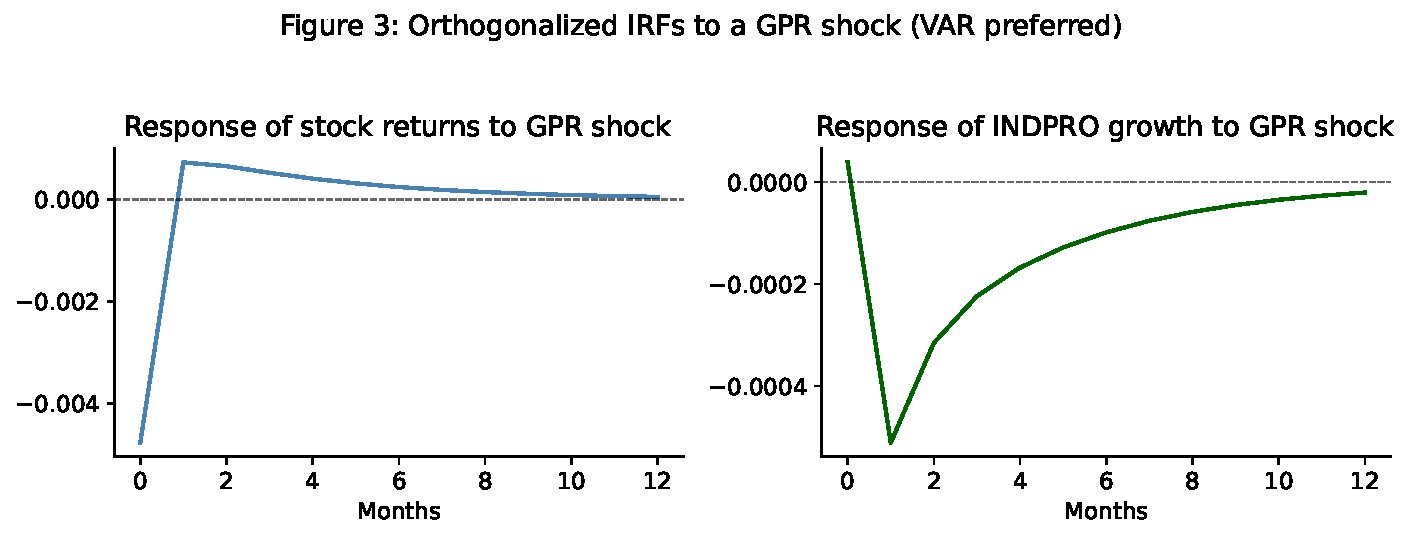
\includegraphics[width=0.95\textwidth]{figures/fig3_irf_orth.pdf}
	\caption{Orthogonalized impulse responses from the preferred VAR(1) with Cholesky ordering $(g,s,y)$.}
	\label{fig:irf_main}
\end{figure}

Robustness checks (not all shown in main output pages) were run for a post-9/11 sample and for a sample excluding 2020--2024. The baseline conclusions are qualitatively unchanged: the $g\rightarrow s$ and $g\rightarrow y$ predictive channels remain statistically weak, while the direct stock-return channel into activity remains the most stable result.
% ─────────────────────────────────────────────────────────────────────────────



% ─────────────────────────────────────────────────────────────────────────────
\section{Discussion}
% ─────────────────────────────────────────────────────────────────────────────
The main strength of the approach is transparency: a small, interpretable VAR directly addresses the assignment question and allows clear testing of predictive and dynamic relationships. The main weakness is that a three-variable reduced-form system cannot capture all channels emphasized in larger macro-financial GPR models. Omitted variables may absorb part of the true transmission mechanism.

Misspecification evidence (heteroskedasticity and non-normality) also matters. It does not invalidate the exercise, but it reduces confidence in strict Gaussian inference and suggests that robust standard errors and careful language are appropriate when discussing significance. In addition, the COVID episode is extreme in monthly macro data and can influence both diagnostics and impulse-response magnitudes.

Finally, Cholesky identification is a maintained assumption. Ordering GPR first is economically plausible and aligned with course material, but contemporaneous restrictions are not directly testable in this setup.



% ─────────────────────────────────────────────────────────────────────────────
\section{Conclusion}
% ─────────────────────────────────────────────────────────────────────────────

Using monthly data from 1985--2025, I estimated a parsimonious VAR for geopolitical risk, stock returns, and U.S. industrial production growth. The preferred model is VAR(1) by BIC. The empirical evidence indicates that stock returns help predict subsequent industrial production growth, while lagged geopolitical risk does not significantly improve prediction of returns or activity in this specification.

Impulse responses suggest an immediate negative stock-market reaction to a geopolitical risk shock, with limited persistence and weak real-activity effects in this small system. Robustness checks across sample choices preserve the broad conclusion. Overall, the findings support a view where financial variables are the strongest short-run transmission channel, while direct monthly predictive effects from aggregate GPR to activity are modest once stock returns are included.


\end{document}